Some 7,000 pages of Clinton's emails were released by the State Department in PDF format \cite{kaggle:emails}.
Kaggle then scraped the text from these PDFs and hosted them as CSVs and SQL databases on the Kaggle Kernels platform.
The dataset contains nearly 8,000 emails sent within Clinton's inner circle from December 2010 to September 2012.
In CSV format, the dataset weighs in at just under 7 MB.

\begin{figure}[h]
  \centering
  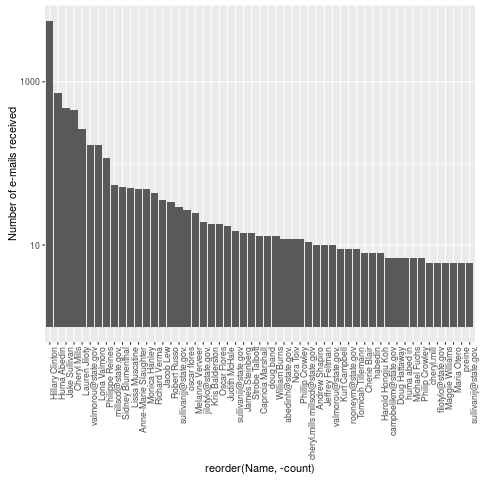
\includegraphics[scale=0.8]{palmer/graphics/num_recvd_histogram}
  \caption{Histogram of how many emails some person has received}
  \label{fig:n_recv_hist}
\end{figure}

\begin{figure}[h]
  \centering
  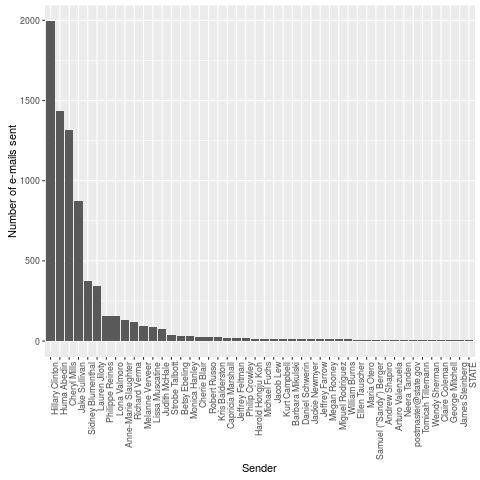
\includegraphics[scale=0.8]{palmer/graphics/num_sent_histogram}
  \caption{Histogram of how many emails some person has sent}
  \label{fig:n_sent_hist}
\end{figure}

Unsurprisingly, the email dataset seems to be Hillary-centric.
In addition, the histogram of emails received seems to be much more highly dispersed than the histogram of emails sent, which may suggest that many emails are sent to multiple people.